\section{Eulerscher Graph}

Ein eulerscher Graph zeichnet sich durch die Existenz eines geschlossenen Pfades aus, der alle Kanten des Graphen genau einmal durchläuft. Diese charakteristische Eigenschaft ist als Eulerkreis bekannt und verleiht dem Graphen eine herausragende Struktur, da er eine systematische Durchquerung aller Verbindungen ermöglicht, ohne eine Kante zu wiederholen \cite{brandstadt1994eulerkreise,liebling1970euler}.

\begin{figure}
    \centering
    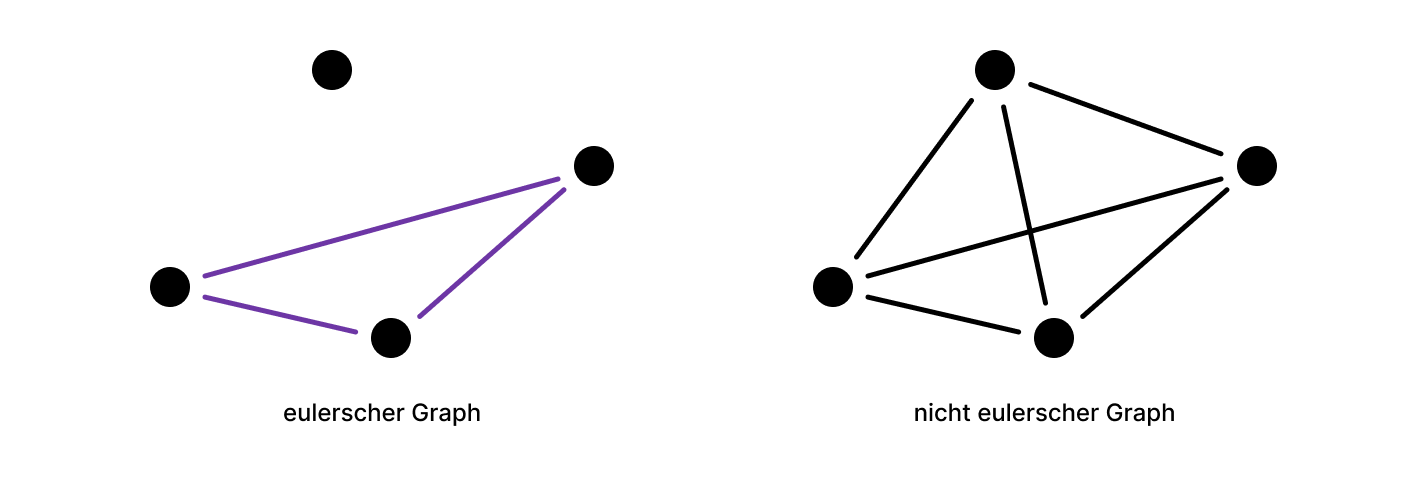
\includegraphics[width=1\textwidth]{content/img/Research/Graphen/EulerscherGraph.png}
    \caption{Graph mit einem Zyklus, welcher alle Kanten einmal enthält (links); Graph ohne diesen Eulerkreis (rechts)}
    \label{fig:eulersche}
\end{figure}
\FloatBarrier